\documentclass{article}
\usepackage{amsmath, amsfonts, amssymb, amsthm}
\usepackage[dvipsnames]{xcolor}

\usepackage[margin=1in]{geometry}
\usepackage{parskip}

% for code sections:
\usepackage[T1]{fontenc}
\usepackage[utf8]{inputenc}
\usepackage[outputdir=../]{minted}
\usepackage{tgadventor} % use a modern font
\usepackage{tcolorbox} % for a box behind the code 
\tcbuselibrary{minted} % tcolorbox library
\usepackage{listings} % to allow for smaller tcblisting font size 
% see https://tex.stackexchange.com/questions/180222/how-to-change-font-size-for-specific-lstlisting 

\setcounter{secnumdepth}{0} % removes section numbering


% Palatino for main text and math
\usepackage[osf,sc]{mathpazo}

% Helvetica for sans serif
% (scaled to match size of Palatino)
\usepackage[scaled=0.90]{helvet}

% Bera Mono for monospaced
% (scaled to match size of Palatino)
\usepackage[scaled=0.85]{beramono}


% % assign zero paragraph indentation — 
% % see: https://tex.stackexchange.com/questions/77999/remove-indent-of-paragraph-and-add-line-skip-with-tufte-latex 
% \makeatletter
% % Paragraph indentation and separation for normal text
% \renewcommand{\@tufte@reset@par}{%
%   \setlength{\RaggedRightParindent}{0pc}%
%   \setlength{\JustifyingParindent}{0pc}%
%   \setlength{\parindent}{0pc}%
%   \setlength{\parskip}{0pt}%
% }
% \@tufte@reset@par
% 
% % Paragraph indentation and separation for marginal text
% \renewcommand{\@tufte@margin@par}{%
%   \setlength{\RaggedRightParindent}{0pc}%
%   \setlength{\JustifyingParindent}{0pc}%
%   \setlength{\parindent}{0pc}%
%   \setlength{\parskip}{0pt}%
% }
% \makeatother

\title{The Central Role of Propensity Scores}

\author{Christian Testa}
\date{August 2023}

% create conditionally independent symbol:
\newcommand\independent{\protect\mathpalette{\protect\independenT}{\perp}}
\def\independenT#1#2{\mathrel{\rlap{$#1#2$}\mkern2mu{#1#2}}}

% vocab command
\newcommand{\vocab}[1]{\textcolor{PineGreen}{\textbf{#1}}}

\newcommand{\E}[0]{\mathbb E}



\begin{document}
\maketitle

{\Large Notes on \textit{The Central Role of the Propensity Score in Observational Studies for Causal Effects} by Paul R. Rosenbaum and Donald B. Rubin (1983), Biometrika}

\section{Introduction}


This paper introduces the reader to the 
propensity score and shows how, through large and
small sample theory, that adjustment
for the scalar propensity score is sufficient
to remove bias due to the observed covariates. 

The quantity of fundamental interest is the 
\vocab{average treatment effect} (presented in their notation): 

$$E(r_1) - E(r_0),$$
where $r_1$ is the outcome under treatment and 
$r_0$ is the outcome under no treatment. 

They introduce \vocab{balancing scores} which are functions $b(x)$ such that 
$$x \independent z | b(x) \quad (\text{or equivalently} \quad  z \independent x | b(x)).$$

In other words, $P(Z|X,b(X)) = P(Z|b(X))$.

We define the \vocab{propensity score} to be 
$$e(x) = Pr(Z=1|X = x) \quad \text{e.g., the probability of treatment given covariates},$$
is the propensity score or propensity towards treatment. 

\subsection{An Example}

We might have a situation where age
is correlated with assignment to the treatment
mechanism. 

Denoting $X$ as age and $Z$ as treatment, consider the following scenario where we set 

$$X \sim \text{Uniform on } \mathbb N \cap \text{ the age range } [19,64]$$
$$Z \sim \text{Bernoulli}(\underbrace{\text{logistic}(\underbrace{\beta_0 + \beta_1 \cdot X}_{\text{log odds}})}_{\text{probability scale}})$$
$$ \text{where logistic}(x) = \frac{1}{1+e^{-x}} = \frac{e^x}{1+e^x}$$

It's clear that $X$ and $Z$ will be dependent and correlated, but by stratifying
on propensity scores estimated via a logistic regression model, we can show 
how conditioning on propensity scores renders $X$ and $Z$ conditionally independent.

% code listing for sampling from a multivariate normal distribution
\begin{tcblisting}{
  listing engine=minted, 
  minted style=friendly, 
  minted language=r, 
  minted options={fontsize=\footnotesize}, 
  colback=lightgray!20, 
  title=R Code for Biased Treatment and Propensity Scoring, 
  listing only
  }
# Dependencies
library(tidyverse)

# Generate a data.frame of 50 folks with ages from 19-65
df <- data.frame(x = sample(x=seq(19,65), replace=TRUE, size = 100))

# Coefficients for our logistic model
beta_0 <- -5
beta_1 <- 0.1

# Compute the odds of treatment using a logistic function
df$e_x <- exp(beta_0 + beta_1 * df$x) / (1 + exp(beta_0 + beta_1 * df$x))

# Assign treatment group based on the computed odds
df$z <- rbinom(n = nrow(df), size = 1, prob = df$e_x)

# Fit a logistic regression model 
model <- glm(z ~ x, data = df, family = binomial(link=logit))

# Report model estimates
coef(model)

# Predicted propensity scores
df$propensity_scores <- predict(model, type="response")

# We can confirm these match our intuition — 
# This is just applying the logistic function 1/(1+exp(-x)) to the
# expanded terms from our regression model.
all.equal(df$propensity_scores, 1/(1+exp(-(coef(model)[1] + coef(model)[2]*df$x))))

# Plot our age-treatment relationship
ggplot(df, aes(x = x, y = z)) + 
  geom_jitter(width=0.25, height=0.025, alpha = 0.5) + 
  geom_line(data = 
    data.frame(x = seq(18,65,.1), 
      y = predict(model, newdata = data.frame(x = seq(18,65,.1)), type='response')),
    aes(x = x, y = y),
    color = 'blue') + 
  xlab("Age") + 
  ylab("Treatment, or Treatment Probability") + 
  ggtitle("Distribution of Treatment Assignment by Age and Logistic Model") + 
  theme_bw()


# Divide the data into bins based on the propensity score
df$e_bin <- cut(df$e_x, breaks = seq(0, 1, by = 0.1))

# Calculate the mean age by propensity score in
mean_x_by_bin <- df |> group_by(e_bin, z) |> summarize(x = mean(x))

# Show age by propensity score bins and treatment
ggplot(df, aes(x = e_bin, y = x, color = as.factor(z))) +
  geom_jitter(width=.25, height = .05, alpha = 0.5, size = 1) +
  geom_line(data = mean_x_by_bin, aes(group = z)) +
  labs(title = "Balance Check: Mean Age (Line) by Propensity Score Bin and Treatment Status"),
       x = "Propensity Score Bin",
       y = "Age",
       color = "Treatment Status")
\end{tcblisting}

\begin{figure*}
    \centering
    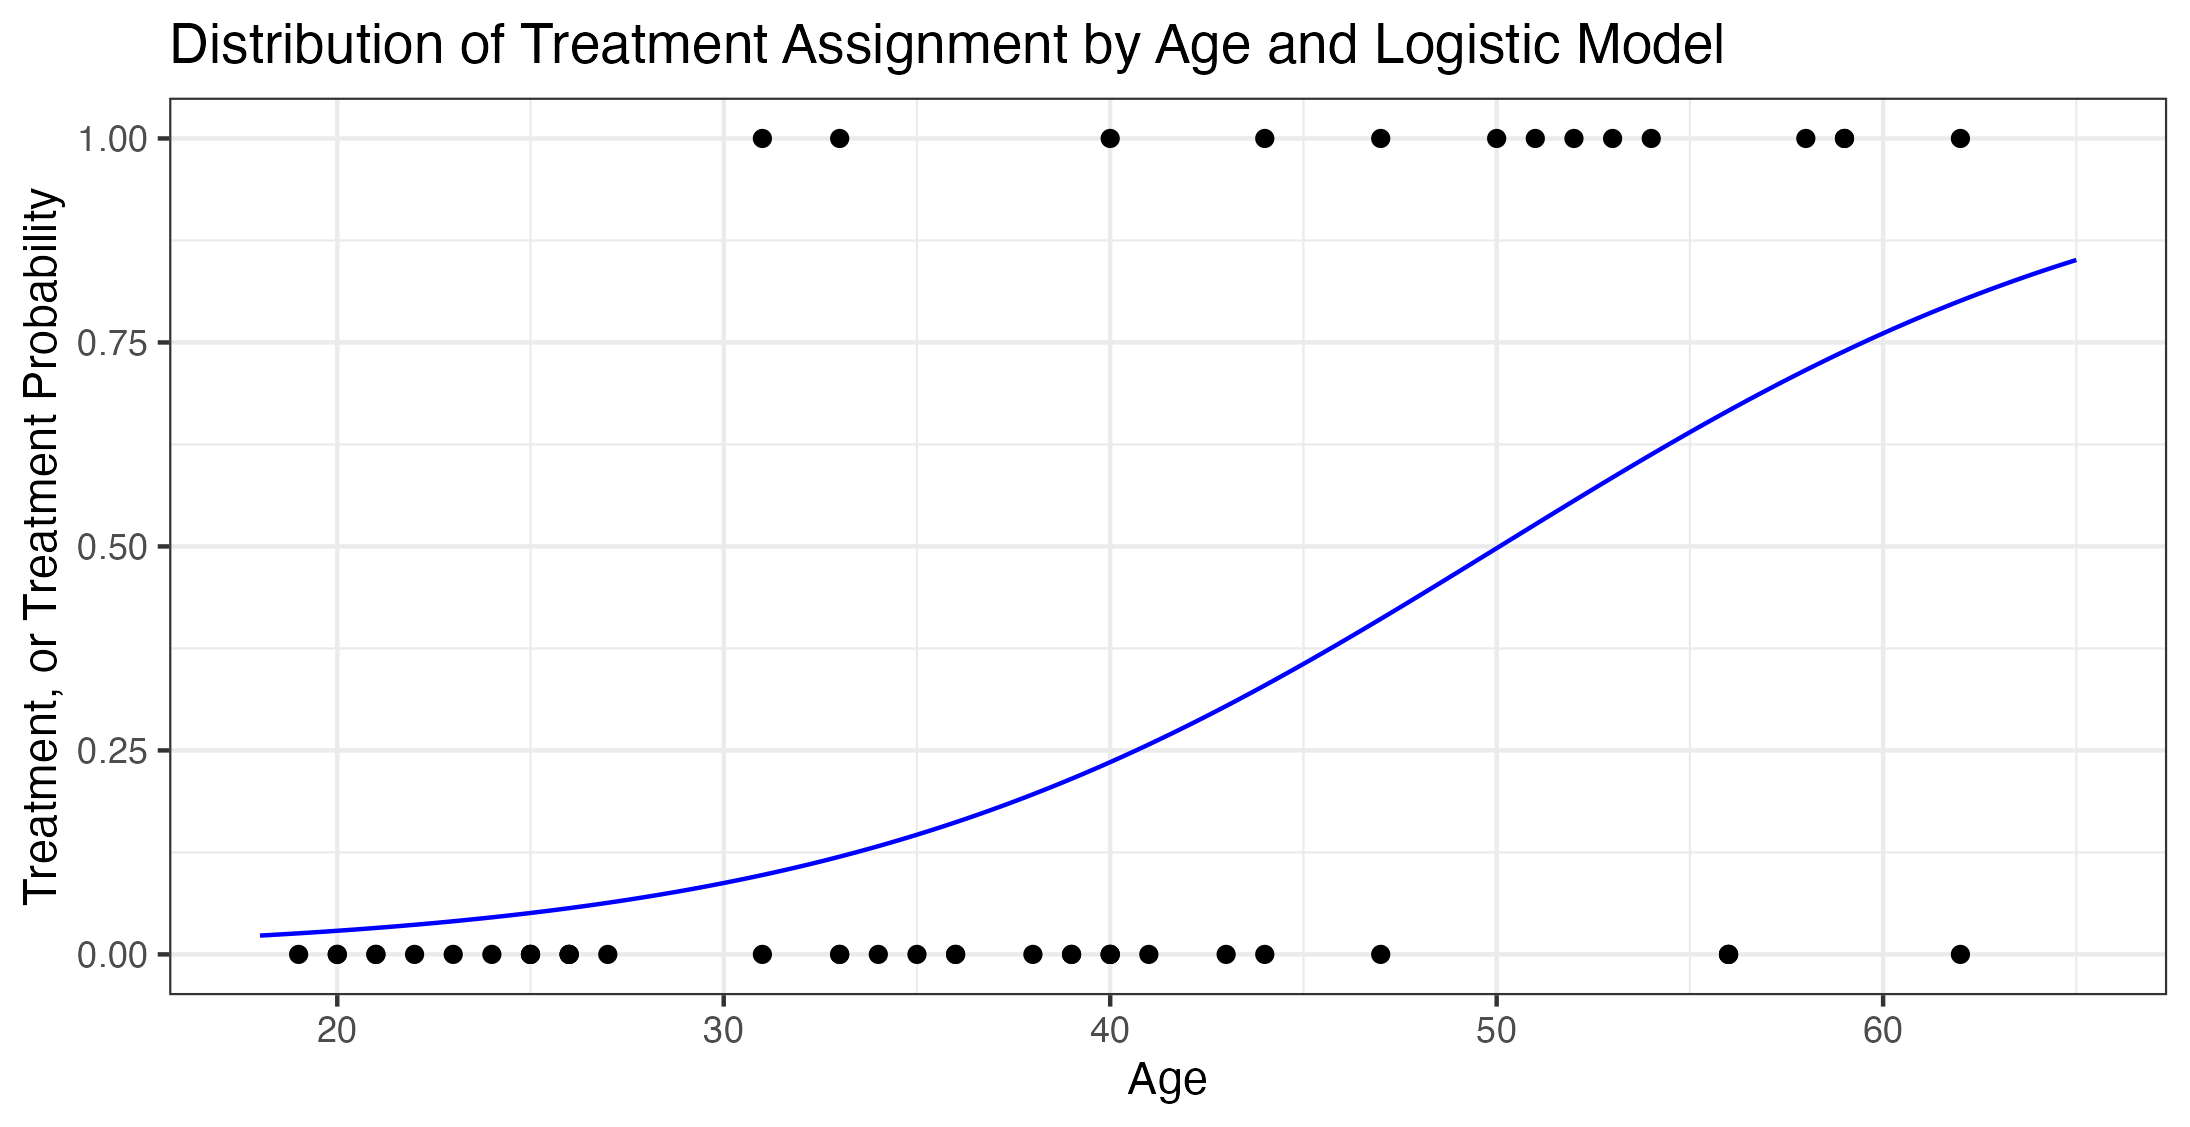
\includegraphics[width=6.5in]{1983 Rosenbaum and Rubin/biased_treatment.png}
    \caption{The distribution of treatment assignment by age and a fit logistic model.}
    \label{fig:treatment_and_logistic}
\end{figure*}

\begin{figure*}
    \centering
    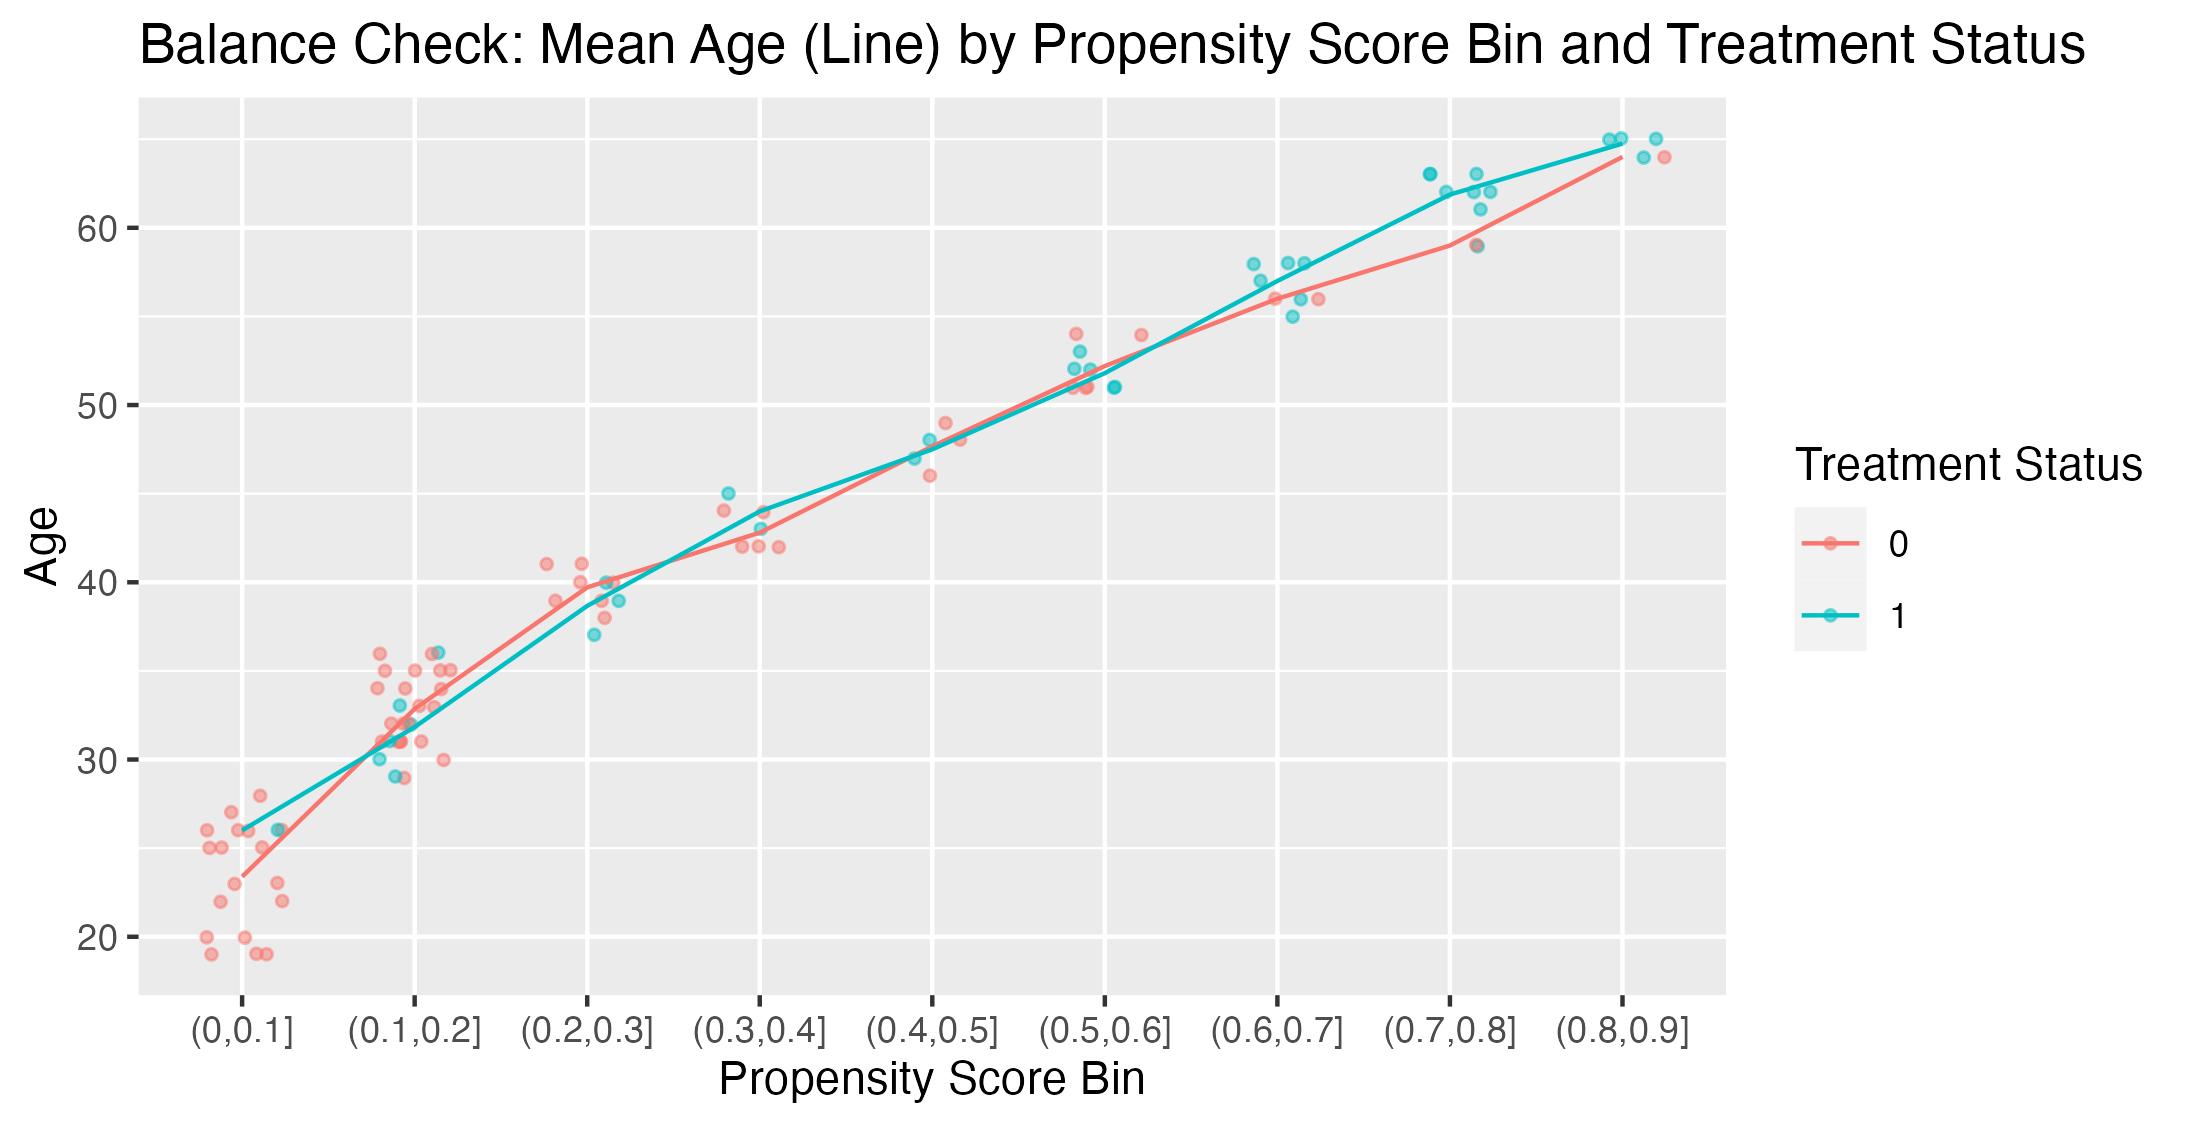
\includegraphics[width=6.5in]{1983 Rosenbaum and Rubin/balance_check.png}
    \caption{A balance check showing that after stratifying by the propensity scores, age and assignment to treatment are independent.}
    \label{fig:balnace_check}
\end{figure*}

\newpage 
\textbf{Theorem 1.} $X \independent Z | e(X)$

This falls out as a special case of Theorem 2, which we will prove in detail.

\textbf{Theorem 2.} Let $b(x)$ be a function of $x$. Then $b(x)$ is a balancing score, that is 
$$x \independent z | b(x)$$
if and only if $b(x)$ is finer than $e(x)$ in the sense that $e(x) = f(b(x))$ for some 
function $f$. 

\begin{proof}
    ($\leftarrow$) First we show that if $b(x)$ is finer than $e(x)$ then it is a balancing score. 
    To show this, it is sufficient to show that $$Pr(Z=1|b(x)) = e(x).$$

    Why is this the case?  Because $e(x)$ is a balancing score, as evidenced by the 
    fact that $Z$ is binary and that $e(x) = Pr(Z=1|X=x)$ completely characterizes the 
    interdependence of $X$ and $Z$.  Given that, conditioning on $e(x)$ is analagous 
    to conditioning on a particular value $X=x$. $X \independent Z \rvert X = x$ is
    of course true given that $x$ is a fixed value independent of $Z$. Similarly 
    we have that $X \independent Z \rvert Pr(Z = 1 | X = x)$. 

    Now we can proceed to show that $b(x)$ is a balancing function by showing that $Pr(Z = 1 | b(x)) = e(x)$. 

    In order to see the truth behind this claim, notice that $e(x)$ is the propensity towards treatment at a given level of covariates $x$ while $Pr(Z=1|b(x))$ is
    the propensity towards treatment among 
    those with covariates that map to $b(x)$ 
    under the function $b$. In other words, we've described the average amount of treatment (or probability) among those with covariates that map to $b(x)$, which can be written $\E[e(x)|b(x)]$. 

    As Rosenbaum and Rubin write it, ``By the definition of $e(x)$, 
    $$ Pr(Z=1|b(x)) = \E[e(x)|b(x)]"$$

    The next step of Rosenbaum and Rubin's is to 
    claim that 
    $$\E[e(X) | b(X) = b(x)] = e(x).$$

    The most straightforward to see this is to start
    by noting that if we fix $X=x$, then any function 
    of $X$ as a random variable also becomes fixed, so that $\E[f(X)|X=x] = f(x)$. In our case, we have that 
    $e(x) = f(b(x))$, so $\E[e(x)|b(x)] = \E[f(b(X))|b(X)=b(x)] = f(b(x)) = e(x)$. 

    As a result, we've shown that 
    $$\mathbb E[e(x)|b(x)] = Pr(Z = 1|b(x)) = e(x),$$
    which concludes this direction of the proof showing that if $b(x)$ is finer than $e(x)$ then it is a balancing score. 
    $$ \exists f \colon e(x) = f(b(x)) \Longrightarrow X \independent Z | b(x).$$

    % Now when we look at the quantity of interest above, 
    % $$Pr(Z=1|b(x)),$$
    % this is essentially asking what is the proportion treated among 
    % all $x$-values with the same level of $b(x)$, or in other words 
    % $\mathbb E[e(x)|b(x)]$. 
% 
    % To see this more rigorously: what we want to establish is that 
    % $$\mathbb E[e(x) | b(x)] = Pr(Z = 1 | b(x))$$
% 
    % Begin by writing that 
    % $$ \mathbb E[e(x) | b(x)] = \mathbb E[Pr(Z=1|X=x)|b(x)]$$
    % Now we can substitute in the conditional probability formula: 
% 
    % $$ = \mathbb E\left[\frac{\int f_{XZ}(Z = 1, X=x) dx }{\int f_X(x) dx } \big\rvert b(X) = b(x)\right]$$
% 
    % $$ = \mathbb E\left[\frac{\int_{x \in b^{-1}(b(x))} f_{XZ}(Z = 1, X=x) dx }{\int_{x \in b^{-1}(b(x))} f_X(x) dx } \right]$$
% 
    % If $b(x)$ is a fixed quantity, this is no longer a random variable
    % and we have that this quantity is exactly $Pr(Z=1 | b(x))$. 
% 
    % As a result, we've shown that 
    % $$\mathbb E[e(x)|b(x)] = Pr(Z = 1|b(x)) = e(x),$$
    % which concludes this direction of the proof showing that if $b(x)$ is finer than $e(x)$ then it is a balancing score. 
    % $$ e(x) = f(b(x)) \Longrightarrow X \independent Z | b(x).$$


    ($\rightarrow$) Moving on, we now prove the converse direction by contradiction.  Suppose that we have $b(x)$, a balancing score such that $X \independent Z | b(x)$, but $b(x)$ is not finer than $e(x)$ so we have $\exists x_1, x_2 \ni e(x_1) \neq e(x_2) \text{ and } b(x_1) = b(x_2)$. 

    We know by applying the definition of $e(\cdot)$ that 
    $$Pr(Z = 1 | X = x_1) \neq Pr(Z = 1 | X = x_2).$$
    However, if $X \independent Z | b(x)$, then we should have that 

    $$Pr(Z = 1 | X = x_1, b(x_1)) = Pr(Z=1 | b(x_1)), \quad \text{ and }$$
    $$Pr(Z = 1 | X = x_2, b(x_2)) = Pr(Z=1 | b(x_2)).$$

    Since $b(x_1) = b(x_2)$, we also then know that 
    $$Pr(Z=1 | b(x_1)) = Pr(Z=1 | b(x_2)),$$
    but this would imploy that 
    $$e(x_1) = Pr(Z = 1 | X = x_1, b(x_1)) = Pr(Z = 1 | X = x_2, b(x_2)) = e(x_2)),$$
    which is a contradiction to our assumption that $e(x_1) \neq e(x_2)$. 

    Thus if $b(x)$ is a balancing function then it must be finer than $e(x)$.
    $$X \independent Z | b(x) \Longrightarrow e(x) = f(b(x)).$$
\end{proof}

\textbf{Definition.} We say that \vocab{treatment assignment} is strongly ignorable given a vector of covariates $v$ iff 
$$(r_1,r_0) \independent z | v, \quad 0 < Pr(Z=1|v) < 1.$$

\textbf{Theorem 3.} If treatment assignment is strongly 
ignorable given $x$, then it is strongly ignorable
given any balancing score $b(x)$; that is,
$$(r_1, r_0) \independent Z | X$$
and
$$0 < Pr(Z=1 | X) < 1$$
for all $x$ imply 
$$(r_1, r_0) \independent Z | b(X)$$
and 
$$0 < Pr(Z = 1 | b(X)) < 1$$
for all $b(X)$.

\begin{proof}
    It is clear that if $0 < Pr(Z = 1|x) < 1$
    for all values of $x$, then there is no 
    such value of $x$ where conditioning on 
    $b(x)$ would push the quantity $Pr(Z=1|b(x))$
    outside the interval $(0,1)$. 

    What remains then is to show that $(r_1, r_0) \independent z | b(x)$, or rewritten that 
    $$Pr(Z=1 | r_1, r_0, b(x)) = Pr(Z=1 | b(x)),$$
    which, if we recall the proof to Theorem 2, we
    have shown $$ = e(x).$$ 

    In order to show the claimed equality, we rewrite
    the probability of treatment given $r_1, r_0,$ and $b(x)$ as the expected value of $Pr(Z=1 | r_1, r_0, X)$ conditioned on $b(x)$. 
    We then have, by the assumption that $(r_1, r_0) \independent Z | X$, 
    $$Pr(Z = 1 | r_1, r_0, b(x)) = \E[Pr(Z=1|r_1,r_0,X)|b(x)] = \E[Pr(Z=1|X)|b(x)] = 
    \E[e(X)|b(x)] = e(x).$$
\end{proof}

\textbf{Theorem 4.} 

\end{document}
